%/*******************************************************************************
% * Copyright (c) 2009, medshare GmbH and Sysmex Digitana AG
% * All rights reserved. This program may not be distributed
% * or modified without prior written consent
% *
% * Contributors:
% *    T. Schaller - initial implementation
% *
% *******************************************************************************/
\documentclass[a4paper]{scrartcl}
\usepackage{german}
\usepackage[utf8]{inputenc}
\usepackage{makeidx}
\usepackage{wrapfig}
\makeindex

\usepackage[pdftex]{graphicx}
\DeclareGraphicsExtensions{.pdf,.jpg,.png}

\usepackage{floatflt}
\usepackage[]{hyperref}
\usepackage{color}
\title{Elexis - Sysmex Connector}
\author{medshare GmbH}

\def\<{{\tt\char'74}}
\def\>{{\tt\char'76}}

\begin{document}

\maketitle
	\begin{center}
		
\includegraphics{elexis_logo}
	\end{center}
	\begin{center}
		
\includegraphics{sysmex_logo}
	\end{center}
	\begin{center}
		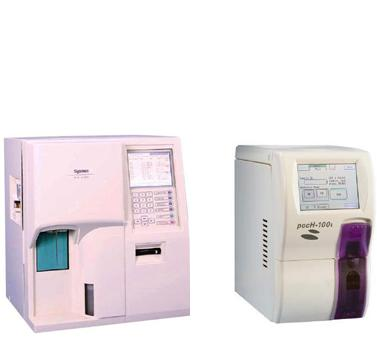
\includegraphics{sysmex_device}
	\end{center}
\pagebreak


\section{Einf\"uhrung}
Dieses Plugin dient dazu, die Laborger\"ate\footnote{Firma Sysmex Digitana} 'Sysmex KX-21', 'Sysmex KX-21N' und 'pocH-100i' an Elexis anzubinden. Mit diesem Plugin k\"onnen die, vom Ger\"at gemessenen Laborparameter direkt in die Elexis-Datenbank eingelesen werden.

\subsection{Voraussetzungen}
Dieses Plugin ben\"otigt Elexis V1.4.1 oder h\"oher sowie ein pocH-100i oder ein Sysmex Ger\"at (Modell KX-21 oder KX-21N). Ausserdem wird ein PC mit mindestens einer freien seriellen Schnittstelle und ein korrekt, gekreuzt verdrahtetes serielles Kabel (Nullmodemkabel) zur Verbindung des Ger\"ates mit dem PC ben\"otigt\footnote{Alternative: RS-232 Adapter f\"ur USB oder Bluetooth}.

\section{Installation und Konfiguration}
Installieren Sie auf dem, sich im Labor befindlichen PC das Plugin wie gewohnt. Verbinden Sie dann bei \textbf{ausgeschalteten} Ger\"aten das Sysmex mit einem seriellen Port des Computers. 
\subsection{Daten\"ubertragung am Sysmex einschalten}
Die serielle Datenkommunikation ist im Sysmex standardm\"assig inaktiv. Damit das Sysmex Ger\"at Daten \"uber die Schnittstelle an den Computer sendet, muss die Daten\"uber-tragung eingeschaltet werden. Wie dies gemacht wird, ist in der Gebrauchsanweisung zum Sysmex beschrieben (z.B. KX-21N: Kapitel 6, Seite 6.9). Es folgt hier nur eine Kurzform f\"ur ge\"ubte Techniker:\\
\\
\textbf{Kommunikationsparameter f\"ur KX-21 und KX-21N:}\\
Select, 6 (Einstellungen), 5 (Labor-EDV-Einst)\\
 - Verbindung: aktiv (mit Pfeiltasten li/re)\\
 - Ausgabeformat: \textbf{K-1000} oder \textbf{KX21N}\\
 - Autom. Ausgabe: On\\
 - Baud-Rate: 9600 (*)\\
 - Code: 8 bits (*)\\
 - Stop-Bit: 1 bit (*)\\
 - Parit\"atspr\"ufung: None (*)\\
 - Protokoll: Class A\\
 - Intervall: 2\\
 - RTS/CTS: Ignore\\
Select, \"Ubern. (mit Pfeiltasten li/re), Enter\\
\\
(*): Empfehlung; eingestellter Wert muss mit Elexis Konfiguration \"ubereinstimmen!\\
\textbf{Kommunikationsparameter f\"ur pocH-100i:}\\
Men\"u, Einstell., Host-\"Ubertragung\\
 - Anschluss: seriell\\
 - Autoausg.: Aktiv\\
 - Format: \textbf{KX-21N}\\
 - \"U-Rate: 9600bps (*)\\
 - Datenl\"an.: 8 bits (*)\\
Pfeil nach rechts\\
 - Stop-Bit: 1 bit (*)\\
 - Parit\"at: Deaktiv. (*)\\
 - Protokoll: Class A\\
 - \"U-Intervall: 2\\
 - RTS/CTS: Deaktiv.\\
Speichern, OK\\
\\
(*): Empfehlung; eingestellter Wert muss mit Elexis Konfiguration \"ubereinstimmen!\\
\\
\subsection{Elexis Konfiguration}
Starten Sie Elexis und gehen Sie dort zu \textsc{Datei-Einstellungen-Datenaustausch-Sysmex} (S. Abb. \ref{fig:config}).
\begin{figure}[h]
    \centering
    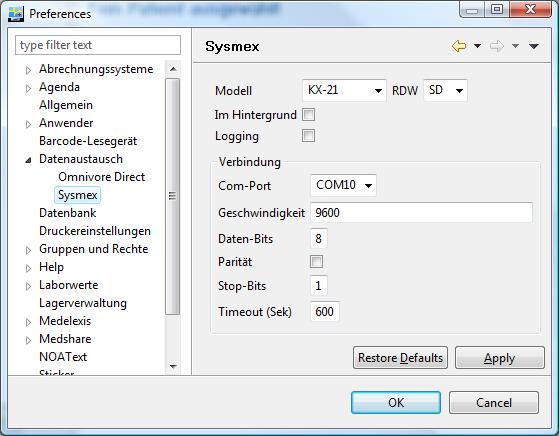
\includegraphics{config}
    \caption{Einstellungen Sysmex}
    \label{fig:config}
\end{figure}
\\
Hier w\"ahlen Sie Ihr Ger\"atemodell (KX-21, KX-21N oder pocH-100i) aus und stellen den seriellen Port, sowie die Schnittstellenparameter ein. Die Werte Geschwindigkeit\footnote{Sysmex: Baud-Rate}, Daten-Bits\footnote{Sysmex: Code}, Parit\"at\footnote{Sysmex: Parit\"atspr\"ufung} und Stop-Bits\footnote{Sysmex: Stop-Bit} m\"ussen mit den Einstellungen auf dem Sysmex Ger\"at \"ubereinstimmen (siehe vorheriges Kapitel).\\
\\
Spezialfall KX-21:\\
Hier m\"ussen Sie in der Auswahlliste 'RDW' angeben, ob das Ger\"at den Wert RDW als SD oder CV liefert\footnote{Sysmex: Kann auf dem KX-21 Ger\"at folgendermassen eingestellt werden: Select, 6, 1}\\
\\
\textbf{Weitere Konfigurationswerte:}\\
\textbf{Timeout (Sek):} Der Wert bestimmt, wie lange Elexis maximal auf Resultate warten soll, bevor die Verbindung getrennt wird.\\
\\
\textbf{Im Hintergrund:} Damit beeinflussen Sie das Verhalten von Elexis. Bei eingeschalteter Option wird die \"Ubertragung im Hintergrund ausgef\"uhrt und Sie k\"onnen weiter in Elexis arbeiten. Bei ausgeschalteter Option erscheint die Abb. \ref{fig:connected}\\
\\
\textbf{Logging:} Diese Option verwenden Sie bitte nur auf Anweisung des Supports, ansonsten wird Ihr Computer mit unn\"otigen Daten gef\"ullt.\\
\section{Verwendung}
Wenn das Plugin korrekt installiert ist, erscheint in der Labor-View automatisch ein neuer Toolbar Button 'Sysmex' (Abb. \ref{fig:toolbarbutton}). Klicken Sie auf diesen Knopf um die Verbindung mit dem Ger\"at herzustellen. 
\begin{figure}[h]
    \centering
    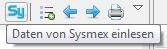
\includegraphics{toolbarbutton}
    \caption{Sysmex Daten einlesen}
    \label{fig:toolbarbutton}
\end{figure}
Die Verbindung bleibt bestehen bis ein Wert \"uber-tragen wurde oder das Timeout gem\"ass Konfiguration abgelaufen ist. Das Sysmex Ger\"at ben\"otigt f\"ur die Tests ca. 45 Sekunden. Jedesmal wenn ein Test abgeschlossen ist, wird das Resultat an den Computer gesendet.\\
\\
\textbf{Wichtig:} Der PC muss dabei auf Empfang sein, ansonsten erscheint auf dem Ger\"at eine Fehlermeldung\footnote{Sysmex: Piepston kann mit 'C' abgeschaltet werden. Dar\"uber hinaus muss danach aber die automatische \"Ubertragung aus- und wieder eingeschaltet werden. Siehe dazu Kapitel 'Installation und Konfiguration'}.
Nach der \"Ubertragung eines Messresultates bleibt die Schnittstelle noch f\"ur 5 Sekunden aktiv (dies f\"ur den Fall, dass manuell mehrere Werte auf dem Ger\"at f\"ur die \"Ubertragung selektiert wurden). Anschliessend wird die Schnittstelle beendet und muss vor der n\"achsten Messung erneut eingeschaltet werden.
\begin{figure}[h]
    \centering
    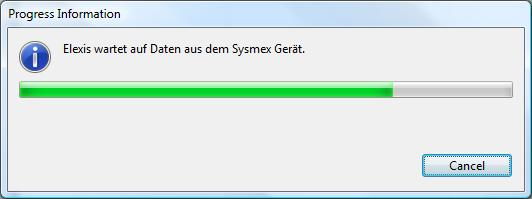
\includegraphics{connected}
    \caption{Verbindung zum Sysmex ist aufgebaut}
    \label{fig:connected}
\end{figure}
Wenn Elexis ein Resultat empf\"angt, muss der Anwender dieses einem Patienten zuordnen. Dazu wird das Elexis Fenster f\"ur die Patientenselektion angezeigt.\\
\\
Es kann passieren, dass die Daten\"ubetragung zwischen Sysmex und Computer fehlschl\"agt. In diesem Fall kann ein oder mehrere Messwerte auf dem Sysmex folgendermassen erneut gesendet werden (siehe n\"achstes Kapitel).\\

\subsection{Messwerte erneut senden}
\textbf{Sysmex KX-21:}\\
Select, 1 (Datenspeicher)\\
Mit Pfeiltasten (nach oben/unten) zum gew\"unschten Messwert navigieren\\
Enter zum Selektieren des Messerts f\"ur die \"Ubertragung (es k\"onnen mehrere Messwerte selektiert werden)\\
3 (Labor-EDV)\\
\\
\textbf{Sysmex KX-21N:}\\
Select, 1 (Datenspeicher)\\
Mit Pfeiltasten (nach oben/unten) zum gew\"unschten Messwert navigieren\\
Enter zum Selektieren des Messerts f\"ur die \"Ubertragung (es k\"onnen mehrere Messwerte selektiert werden)\\
2 (Ausgabe)\\
1 (Host)\\
\\
\textbf{pocH-100i:}\\
Men\"u\\
Datensp.\\
Mit Pfeiltasten (nach oben/unten) zum gew\"unschten Messwert navigieren\\
Host\\
\section{Plattformen}
Dieses Plugin wurde unter Windows XP und Vista getestet. Beachten Sie bitte, dass unter Linux die seriellen Ports nicht COM1 usw., sondern /dev/ttyS0 usw. heissen.
\section{Kabelspezifikation}
\begin{figure}[h]
    \centering
    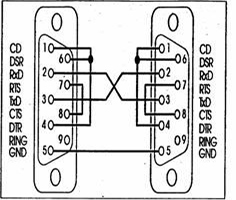
\includegraphics{kabel}
    \caption{Sysmex Kabelkonfiguration}
    \label{fig:kabel}
\end{figure}
Es wird ein gekreuztes, serielles Kabel ben\"otigt (Nullmodemkabel! gem\"ass Abb. \ref{fig:kabel})). Das Kabel muss an beiden Enden einen 9-poligen Stecker (weiblich) aufweisen.
\end{document}
